\clearpage % clear the prior chapter's page

\chapter{Related Work}\label{CH2_RelatedWork}
%\vspace{-7mm}
%\bigskip

\section{DD and HDD}
There are several different algorithms used to simplify unit tests or code bases. One of which is DD, an algorithm that simplifies failing tests while still keeping the bug. This algorithm works by utilizing a variant of binary search to remove individual components that are unnecessary for triggering the bug~\cite{zeller2002simplifying}. To retrofit DD for hierarchical test inputs like XML, HTML, or programs, the top syntax tree is used as a flat structure. This means the elements would include blocks of nested elements for removal. This method is faster and more efficient than other algorithms since it doesn't entail further nested elements but means that it is much more limited since it cannot find further unneeded statements within deeper code blocks. It cannot find these statements because the algorithm treats these code blocks as a single statement, meaning it removes the entirety of the block or none at all. This is relevant since many algorithms that need to be reduced have tree-like structures, meaning this algorithm cannot effectively simplify every test.

The DD algorithm works by separating a portion of code into smaller sections. By testing these sections in certain ways, we are able to find statements that do not need to be kept for the failing logic to remain. If we remove these statements and continue the process until no more statements can be removed, we will end up with the simplified failing test. We start with a certain number of sections and test each individually. If any of these tests fail, we use that as the new input. If all of these sections' tests succeed or cannot compile, we continue searching. After testing each of these, we will test the compliment of each section, or the combination of every other section. Likewise, if we find a failing configuration, we use that as the new input. If all of these configurations fail, we increase the granularity until the number of sections exceeds the number of statements remaining.

While DD is useful alone, it is not effective for all situations. One situation was further investigated by Misherghi and Su, who proposed that HDD works effectively on tree-like inputs by exploiting the underlying AST~\cite{misherghi2006hdd}. This AST allows for the HDD algorithm to break down the blocks of code into smaller blocks of code, thus allowing for the algorithm to run recursively and find additional unneeded statements for removal. The primary concern with using this approach comes from the increased time, and therefore more resources, needed to parse these AST structures. While both DD and HDD are theoretically sound algorithms that guarantee convergence and minimalism, HDD is able to break down the statements further, allowing for more effective simplification. 

The HDD algorithm is useful for finding and reducing code and tests within a tree structure. This algorithm works by breaking down the statements recursively by blocks of code. It then runs the DD algorithm at every level in a postorder traversal, or in other words, it starts with the inner-most layer. If a block needs to be removed entirely, it will do so while simplifying a layer above it. Take a look at figure~\ref{fig:hddFigure} for pseudo-code behind the HDD algorithm.

\begin{center}
\begin{figure}[!ht]
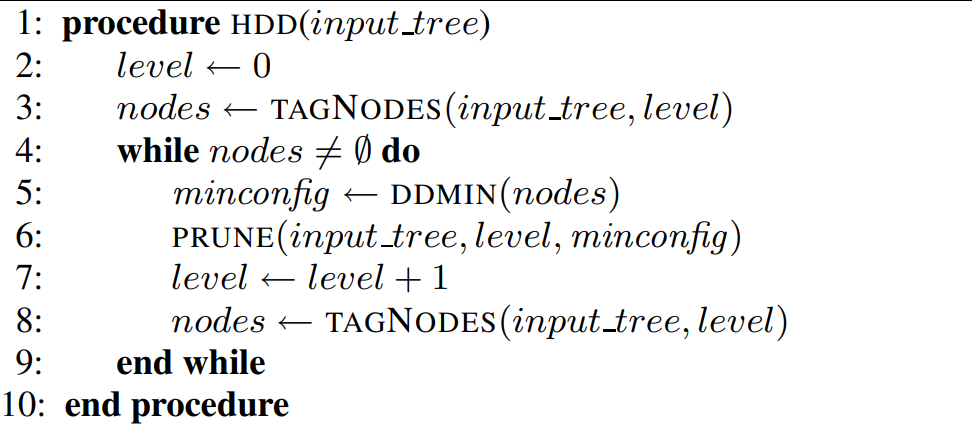
\includegraphics[width=\linewidth]{hddFigure.png}
\caption{HDD algorithm~\cite{misherghi2006hdd}}
\label{fig:hddFigure}
\end{figure}
\end{center}

Regehr et al. proposed C-Reduce to simplify tests for C compiler testing that uses DD as a starting point and further generalizes it. They also look into the test case validity problem to handle undefined and unspecified behavior. Their work showed significant improvement in simplifying C compiler tests that were produced by C-Smith (a random testing tool for C compiler testing) compared to other approaches~\cite{regehr2012test}.

Fuzzers are random testing mechanisms. When fuzzers are used to find bugs, they tend to find the same bugs repetitively. This makes it harder to find diverse bugs early. Fuzzer taming is used to make fuzzers produce more diverse bugs early or to categorize the bugs such that different bugs fall into different categories. Pei et al. combined delta-debugging trails with Furthest Point First algorithm to produce diverse bugs early~\cite{7022682}.

While simplifying tests with DD algorithms can help find underlying bugs in code bases, it still needs existing tests to be able to catch these bugs. Alex Groce et al. avoids this limitation with \emph{cause reduction}~\cite{groce_alipour_zhang_chen_regehr}. \emph{Cause reduction} utilizes the DD algorithm to simplify test cases with respect to arbitrary effects in order to provide quick tests for real-world programs. In other words, \emph{cause reduction} can help find bugs by exploring additional branches of variants that normally would not be explored by the regular DD algorithms. These additional variants provide more areas for potential bugs without a need for a unit test. Therefore, this has the potential to be more effective at finding bugs than previous approaches. 

\section{Additional resources}
Even though HDD was able to create a tree structure, it did not do anything about changing the structure of the syntax tree. This would lead the tree to be imbalanced at times, making a situation not ideal for the HDD algorithm. Using this algorithm with an unbalanced tree is inefficient and resource intensive. This led Hodovan and Kiss to research further, and claim that Extended Context Free Grammar with HDD produces a more balanced tree than one produced by a Context Free Grammar. In other words, by changing the way these statements are parsed, it can create a more balanced tree, leading to a more efficient situation. They then utilized it in implementing a modernized HDD tool called picireny~\cite{hodovan2016modernizing}. 

While the DD and HDD algorithms are effective with simplification, there is potential for better algorithms. In order to have both effectiveness and efficiency, you need to implement both algorithms, and this will still only provide one benefit or the other. In an effort to address this issue, Herfert et al. proposed an additional algorithm known as the Generalized Tree Reduction (GTR) algorithm. The GTR algorithm relies on operations other than removal or deletion and replacing a tree node with a similar tree node~\cite{Herfert2017GTR}. This presented an effective alternative to DD and presented the idea that DD/HDD is not the only syntax tree simplification option. This different approach to the problem is a great demonstration that there are still many potential improvements that have not been discovered yet. 

While all these resources find ways of providing alternatives or different approaches to the HDD algorithm, there are still plenty of other areas for performance boosts. These algorithms are slow and resource intensive, and in need of performance enhancements. Sun et al. noticed this issue which led them to research further. They observed that during the simplification process, many previous algorithms produced \emph{syntactically invalid variants}. These \emph{syntactically invalid variants} are variations of the code that will not even pass a simple compilation step. However, a futile compilation step still needs to be performed before pruning the invalid variant. They proposed the \emph{Perses} algorithm specifically to avoid generation of these invalid variants~\cite{perses}. By knowing about these \emph{syntactically invalid variants} before compiling, it makes the application of these algorithms more time efficient since it reduces the amount of time compiling each variant.

While the DD and HDD algorithms provide a solution for test simplification, there are still other enhancements that can be made. Gopinath et al. utilized the \emph{Perses} algorithm to propose the \emph{DDSET} algorithm to abstract minimal failure-inducing input from a larger set using input grammar~\cite{gopinath2020abstracting} creating an additional simplification algorithm. This new algorithm is very efficient and reduces time needed to simplify. This is a very unique approach to the problem and gives another alternative for unit test simplification through generalization of the algorithm and only allowing \emph{syntactically valid} variants.

A large problem with the research so far is the level of abstraction with it. There are several different languages that each provide their own syntax, creating issues with each specific language. This led \emph{Picireny}, \emph{Perses}, and \emph{DDSET} to use Antlr, a powerful parser generator, to produce the AST for specific programming languages~\cite{parr}. Antlr provides the ability to produce a parser for several programming languages without creating each individually. This is a significant tool to use for problems regarding programming languages in general since this will provide a parser for each, giving the option to implement these solutions in a variety of languages.

Binkley et al. proposed another useful resource as the \emph{Observational-based Slicing} (ORBS) technique. This technique uses program line deletion as a fundamental operation to slice programs accurately and efficiently~\cite{binkley2014orbs}. This deletes potential slices of the program and observes and compares the behavior of the program before and after deletion. If the program behaves the same in both the original and the slice, then the deletion is kept. While this concept is not very complex, it provides an additional solution to these simplification problems and opens the door for more ideas to be implement.

An additional resource came from Christi et al. when they combined inverted HDD with statement deletion mutation to simplify programs for the purpose of resource adaptations. They argued that reduction is only meaningful and useful at statement level and avoided non-statement level reductions~\cite{christi2017saso, christi2018qrs}. By only focusing on statements specifically instead of lines generated, there are a significant number of skipped variants that will not compile. Non-statement level reductions can lead to partial statements that cannot compile. By focusing on entire statements, we are able to skip these partial statements and increase efficiency. This approach will still reduce and simplify the same, but provides an alternative to not spend time on compilation for these variants. By doing this, they presented the perspective that simplification performance can be efficient by simply focusing on statement reduction.

